\documentclass[runningheads]{llncs}
\usepackage{amsmath}
\usepackage{amsfonts}
\usepackage{bm}
\usepackage{booktabs}
\usepackage[compress]{cite}
\usepackage{color}
\usepackage{graphicx}
\usepackage{hyperref}
\usepackage{physics}

\renewcommand\UrlFont{\color{blue}\rmfamily}

\begin{document}

\title{
    Multiclass Classification with Pegasos
}
\author{Gabriele Cerizza}
\authorrunning{G. Cerizza}

\institute{Università degli Studi di Milano\\
\email{gabriele.cerizza@studenti.unimi.it}\\
\url{https://github.com/gabrielecerizza/smml}}

\maketitle

\section*{Introduction}
\label{sec:introduction}

In this report we detail the results of our experiments on the Pegasos algorithm~\cite{shalev-pegasos-2011} over a multiclass classification task, pursuant to the project specifications set out for the Statistical Methods for Machine Learning course of the Università degli Studi di Milano\footnote{\url{https://cesa-bianchi.di.unimi.it/MSA/index\_21-22.html}}. 

In Section~\ref{sec:dataset} we illustrate the dataset used in the experiments. In Section~\ref{sec:algorithm} we briefly describe the algorithm and its implementation. In Section~\ref{sec:experiments} we show the results of our experiments and provide comments thereon. Finally, Section~\ref{sec:conclusions} contains our concluding remarks. 

\section{Dataset}
\label{sec:dataset}

Our analysis was carried out on the USPS dataset\footnote{\url{https://www.kaggle.com/datasets/bistaumanga/usps-dataset}}, comprising 9298 $16 \times 16$ grayscale images. These images depict handwritten digits ranging from 0 to 9. A sample of these digits can be seen in Figure~\ref{fig:dataset:digits}. The classes do not present severe imbalance issues, as shown in Figure~\ref{fig:dataset:class_counts}.

To gauge the complexity of multiclass classification on this dataset, we performed dimensionality reduction by way of the t-distributed Stochastic Neighbor Embedding (t-SNE)~\cite{maaten-2008-tsne} algorithm and projected the instances onto a two-dimensional space. The result is shown in Figure~\ref{fig:dataset:tsne}. Within this figure the instances are clustered into ten clearly distinguishable groups, thus suggesting that a satisfying classification can be attained.   

The USPS dataset is made available with predetermined training and test sets. In our experiments, however, we merged these sets and proceeded to form our own training and test sets, as illustrated in Section~\ref{sec:experiments}. 

\begin{figure}
  \center
  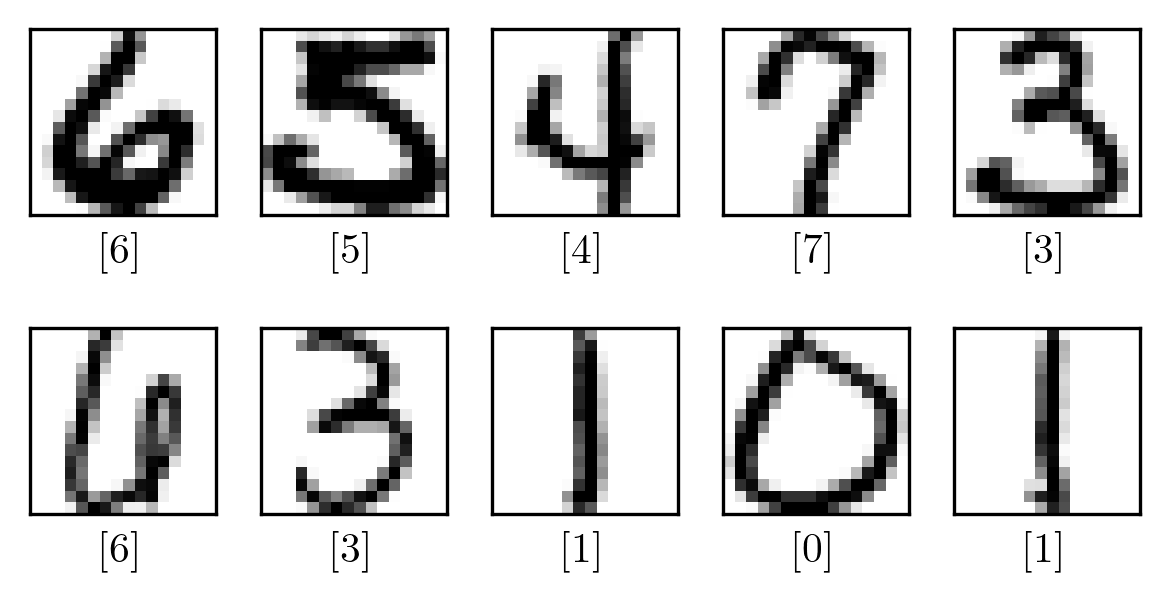
\includegraphics[width=0.7\textwidth]{../img/digits.png}
  \caption{Sample of images from the USPS dataset. The label is indicated below each image.} 
  \label{fig:dataset:digits}
\end{figure}

\begin{figure}
  \center
  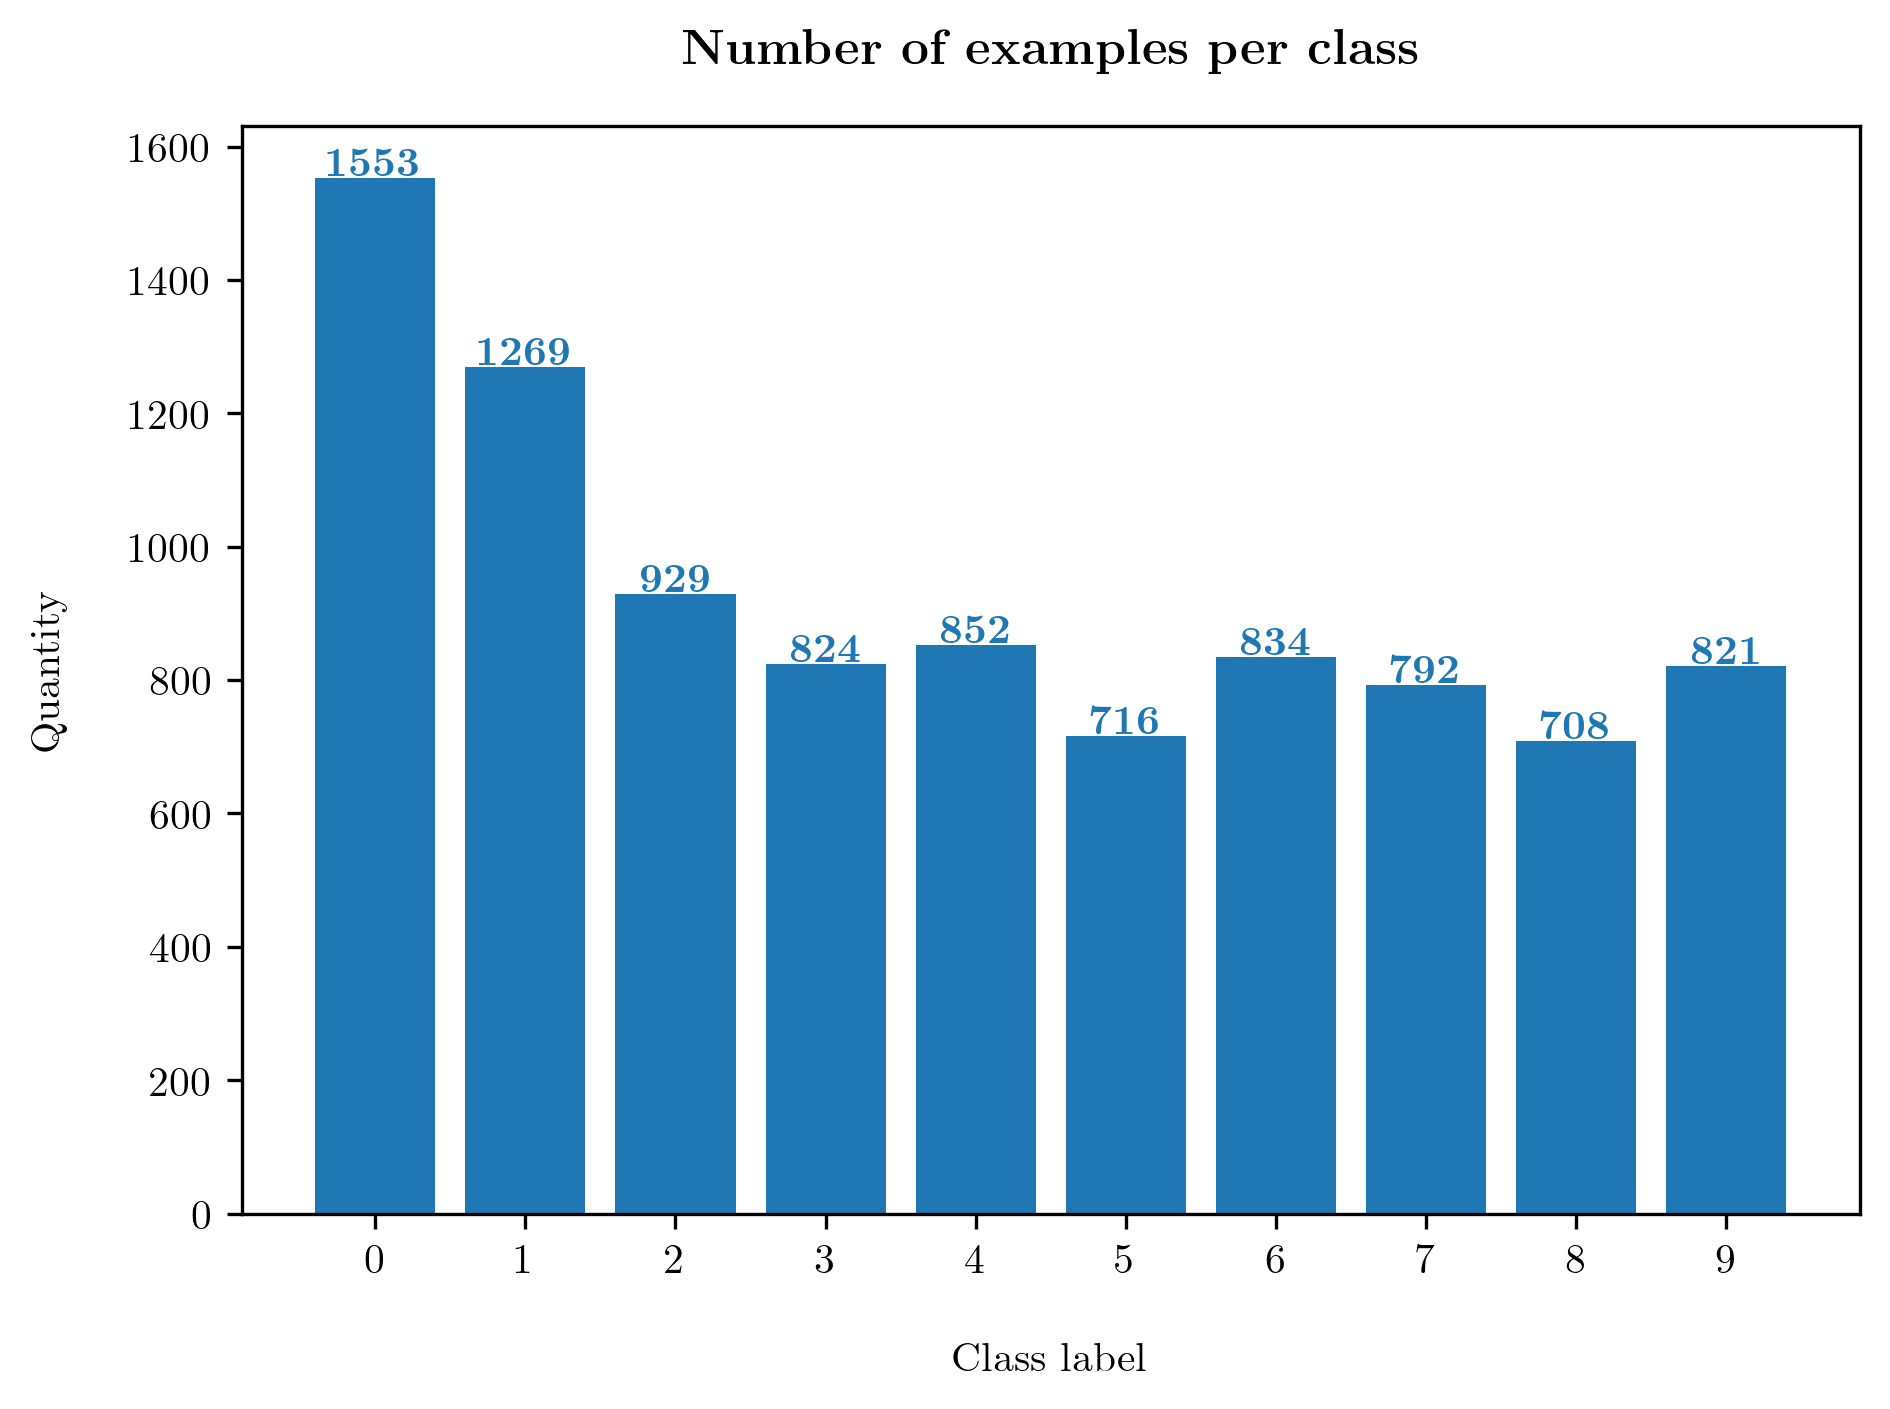
\includegraphics[width=1\textwidth]{../img/class_counts.png}
  \caption{Frequency of the classes in the USPS dataset.} 
  \label{fig:dataset:class_counts}
\end{figure}

\begin{figure}
  \center
  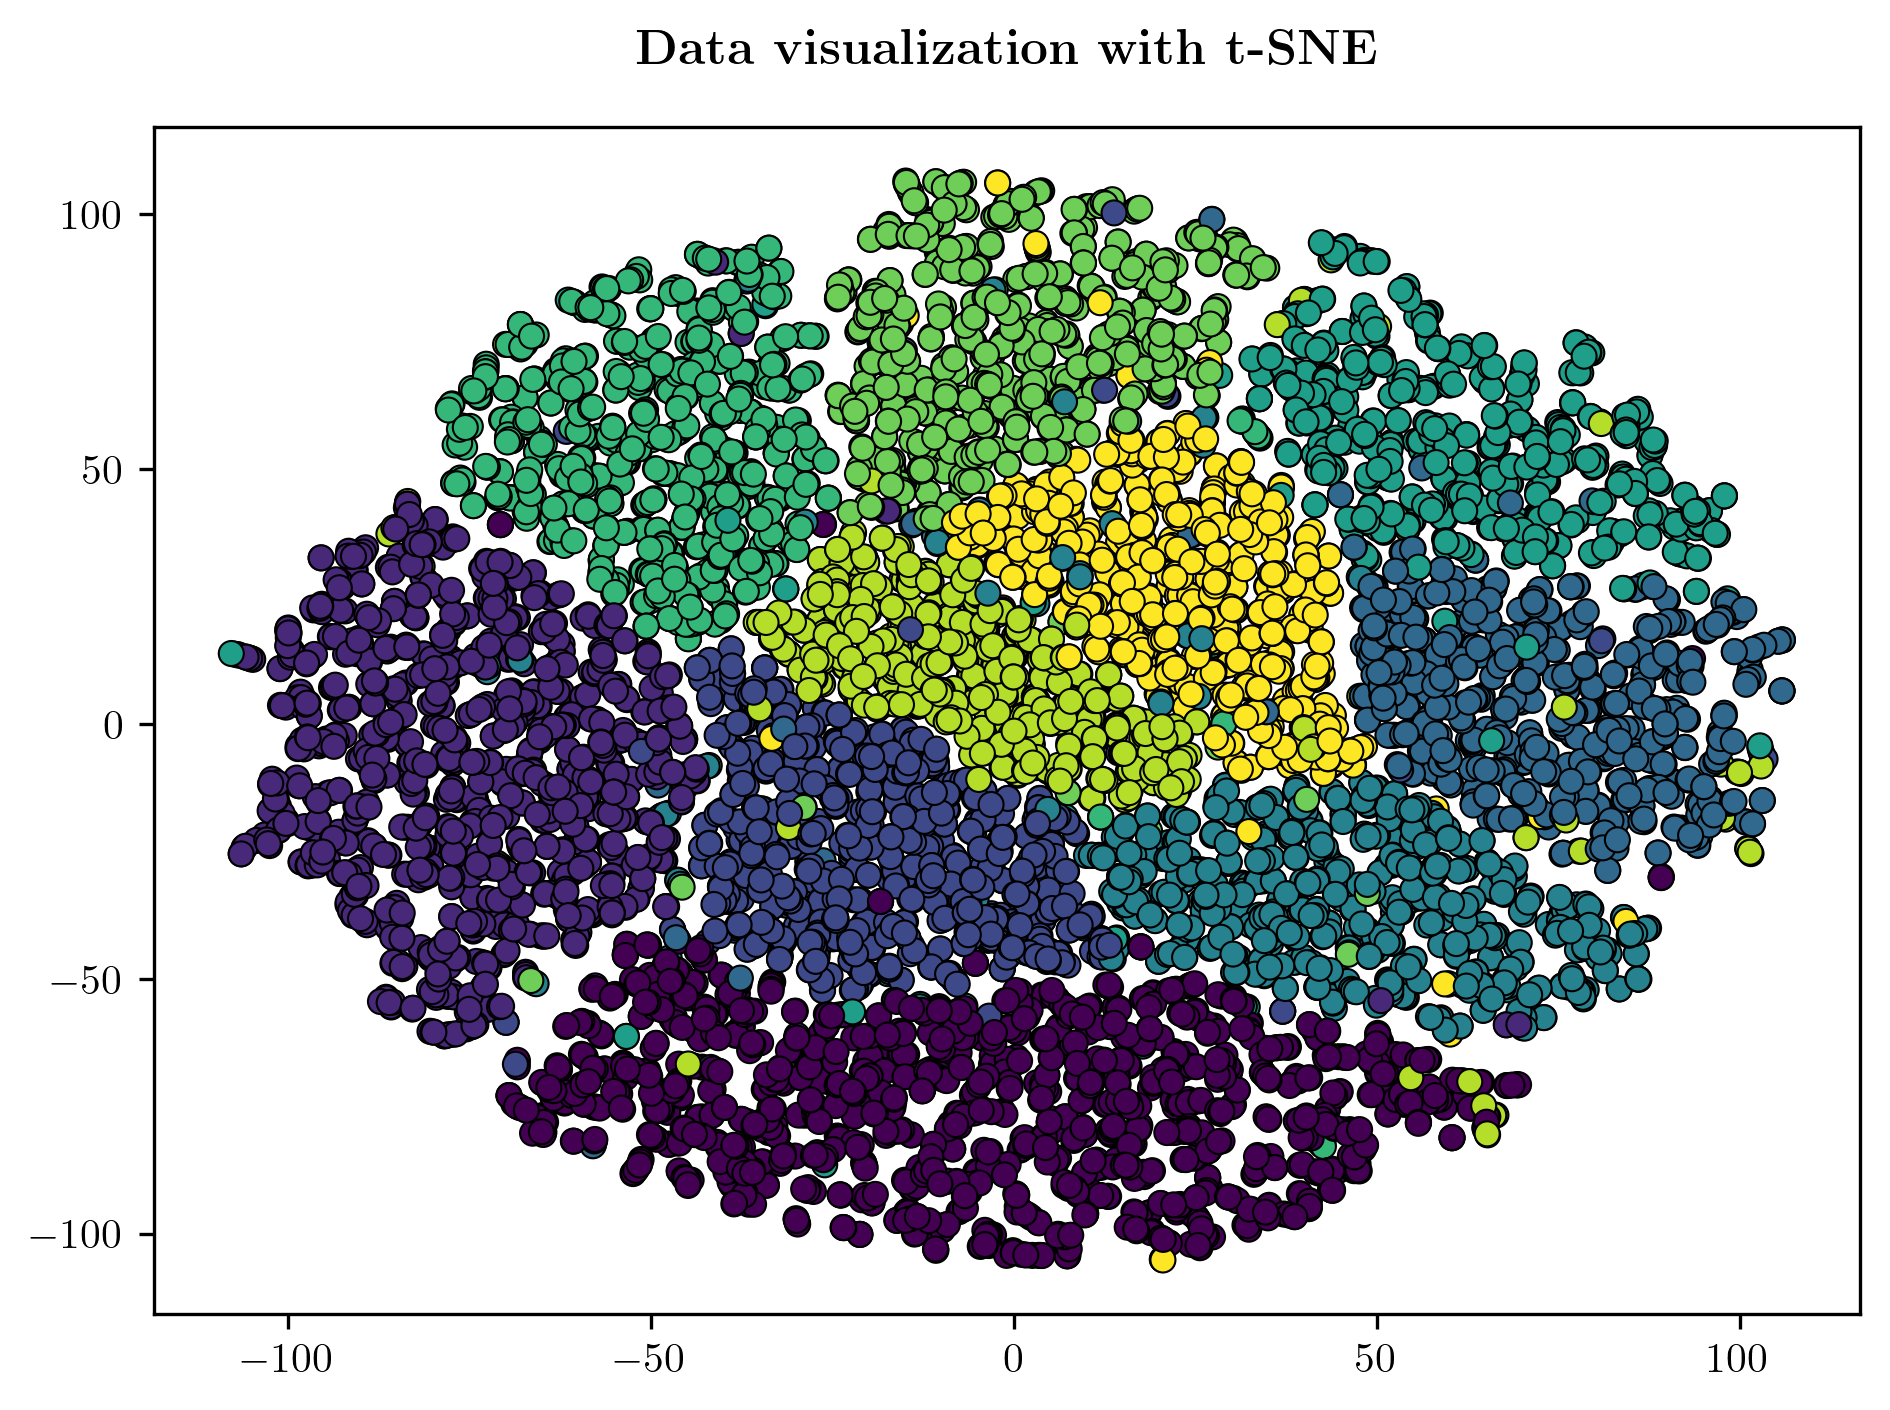
\includegraphics[width=1\textwidth]{../img/tsne.png}
  \caption{Projection of the USPS dataset onto a two-dimensional space using t-SNE.} 
  \label{fig:dataset:tsne}
\end{figure}

\section{Pegasos Algorithm}
\label{sec:algorithm}

In order to perform the multiclass classification task, we employed the Pegasos algorithm~\cite{shalev-pegasos-2011}. This algorithm was introduced to solve the Support Vector Machine (SVM)~\cite{vapnik-1999-statistical-learning} convex optimization problem, which can be formalized as follows. 

Let $S = \{(\bm{x}_1,y_1),\dots,(\bm{x}_m,y_m)\}$ be a training set with $\bm{x}_t \in \mathbb{R}^d \; \forall t=1,\dots,m$; and let $\phi : \mathbb{R}^d \to \mathcal{H}$ be a function such that $\text{dim}(\mathcal{H}) \gg d$. The optimization problem to solve is: 
\begin{alignat}{3}
  &\!\min_{\bm{w} \in \mathbb{R}^d, \bm{\xi} \in \mathbb{R}^m} & \quad & \frac{\lambda}{2} \norm{\bm{w}}^2 + \frac{1}{m}\sum_{t=1}^{m} \xi_t \, , \label{eqn:svm}\\
  &\text{s.t.}  &       & y_t \bm{w}^\top \phi(\bm{x}_t) \geq 1 - \xi_t &\qquad& t = 1,\dots,m \, , \notag\\
  &                   &       & \xi_t \geq 0  &\qquad& t = 1,\dots,m \, , \notag
\end{alignat}
where

Under scrutiny

\section{Experiments}
\label{sec:experiments}

The experiments were run on a machine with 16 GB of
RAM and a CPU Intel(R) Core(TM) i7-9700K 3.60GHz with 8 cores.



\section{Conclusions}
\label{sec:conclusions}

\section*{Statement}
\textit{I/We declare that this material, which I/We now submit for assessment, is entirely my/our own work and has not been taken from the work of others, save and to the extent that such work has been cited and acknowledged within the text of my/our work. I/We understand that plagiarism, collusion, and copying are grave and serious offences in the university and accept the penalties that would be imposed should I engage in plagiarism, collusion or copying. This assignment, or any part of it, has not been previously submitted by me/us or any other person for assessment on this or any other course of study.}


\bibliographystyle{splncs04}
\bibliography{bibtex_entries}

\end{document}